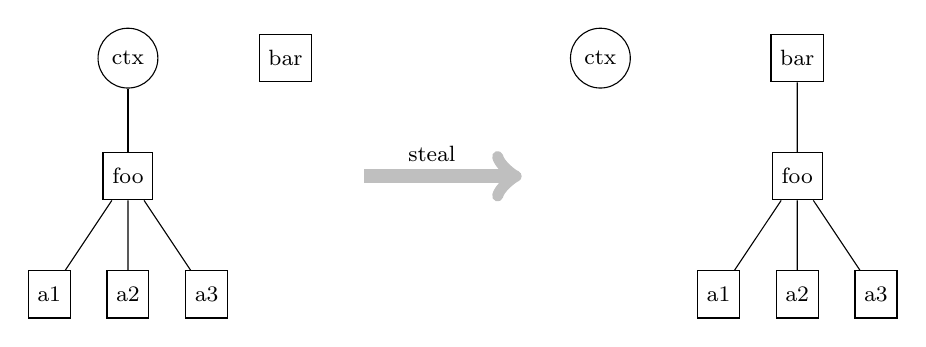
\begin{tikzpicture}
[level/.style={sibling distance=10mm},
 level 1/.style={sibling distance=20mm},
 every node/.style=
   {minimum height=6mm,rectangle,draw=black,font=\footnotesize}]
\begin{scope}
  \node [circle] {ctx}
    child {node [] {foo}
      child {node [] {a1}}
      child {node [] {a2}}
      child {node [] {a3}}
    }
  ;
\end{scope}

\begin{scope}[xshift=2cm]
\node [] {bar};
\end{scope}

\draw [->, line width=5pt, black!25] (3,-1.5) -- 
  node [draw=none,black,yshift=8pt,xshift=-4pt] {steal} (5,-1.5) ;

\begin{scope}[xshift=6cm]
\node [circle] {ctx}
;
\end{scope}

\begin{scope}[xshift=8.5cm]
  \node [] {bar}
    child {node [] {foo}
      child {node [] {a1}}
      child {node [] {a2}}
      child {node [] {a3}}
    }
  ;
\end{scope}
\end{tikzpicture}